This section provides a practical and in-depth introduction to the smart contract programming on the Ethereum blockchain.
Building upon the theoretical foundations laid in the previous section,
we will now transition to the practical aspects of designing,
developing, and deploying smart contracts. The primary focus of this
section will be on Solidity, the most widely adopted programming
language for writing smart contracts on the Ethereum platform.

We will begin by exploring the fundamental elements of the Solidity
language, including its syntax, data types, and control structures. We
will then move on to more advanced topics, such as the use of function
modifiers to create reusable code, the importance of visibility
specifiers for controlling access to functions and state variables, and
the use of libraries to promote code reuse and modularity.

A significant portion of this section will be dedicated to the practical
application of these concepts. We will examine the standards for
creating both fungible (ERC20) and non-fungible (ERC721) tokens, which
are two of the most common use cases for smart contracts on Ethereum.

Finally, we will address the critical topic of smart contract security.
We will discuss common vulnerabilities, such as reentrancy attacks and
integer overflows, and we will explore the best practices and tools that
developers can use to write secure and robust smart contracts. By the
end of this section, you will have the foundational knowledge and
practical skills necessary to begin your journey as a smart contract
developer.

\subsection{Learning Objectives}\label{learning-objectives}

\begin{itemize}
	\tightlist
	\item
	Understand the basics of the Solidity programming language.
	\item
	Learn how to define and interact with smart contracts.
	\item
	Grasp the concepts of visibility specifiers, function modifiers, and
	data locations.
	\item
	Understand the role of fallback and receive functions in handling
	Ether transfers.
	\item
	Learn about the standards for fungible (ERC20) and non-fungible
	(ERC721) tokens.
	\item
	Gain insight into common smart contract vulnerabilities and security
	best practices.
	\item
	Become familiar with the tools and techniques used for smart contract
	development and analysis.
\end{itemize}

\begin{center}\rule{0.5\linewidth}{0.5pt}\end{center}

\subsection{Introduction to
	Solidity}\label{section-1-introduction-to-solidity}

\subsubsection{What is Solidity?}\label{what-is-solidity}

Solidity is a high-level, object-oriented programming language that has
become the de facto standard for writing smart contracts on the Ethereum
blockchain and other EVM-compatible platforms. It is a statically-typed
language with a syntax that is similar to that of JavaScript and C++,
making it relatively easy for developers with experience in these
languages to learn.

The primary purpose of Solidity is to provide a means for developers to
create self-executing contracts that can be deployed to a blockchain.
These contracts can be used to automate a wide range of processes, from
simple token transfers to complex financial instruments.
The users interact with smart contracts through decentralized applications (DAPPs), which run completely server-less -- on the client side (see \autoref{fig:dapps}).


\begin{figure}[t]
	%	\vspace{-0.3cm}
	\begin{center}
		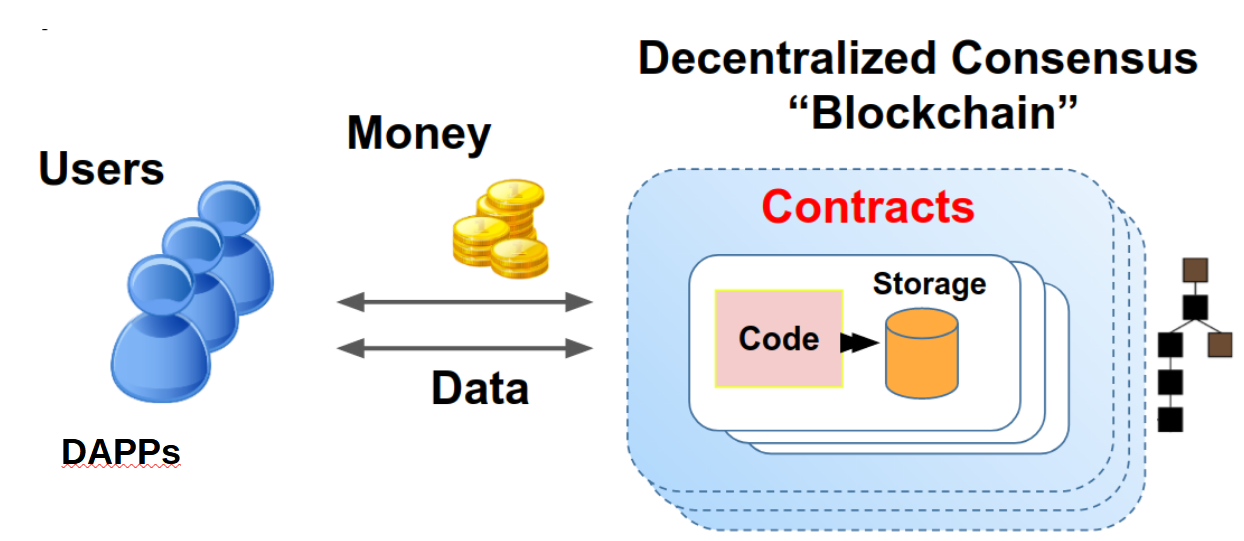
\includegraphics[width=0.8\textwidth]{./figs/smart-contracts-flow.png}
		\caption{Users interacting with smart contract through DAPPs (that run on the client-side).}		
		\label{fig:dapps}
	\end{center}	
\end{figure}
  

\subsubsection{The Structure of a Solidity
	Contract}\label{the-structure-of-a-solidity-contract}

A Solidity contract is a collection of code and data that is deployed to
a specific address on the blockchain. It is analogous to a class in an
object-oriented programming language, in that it encapsulates both data
(in the form of state variables) and behavior (in the form of
functions).

A typical Solidity source file has the following structure:

\begin{itemize}
	\tightlist
	\item
	\textbf{Pragma Directive}: This is a declaration that specifies the
	version of the Solidity compiler that should be used to compile the
	code. This is important for ensuring that the code is compiled
	correctly and that it is compatible with the target version of the
	EVM.
	\item
	\textbf{License Identifier}: This is a comment that specifies the
	license under which the code is released. This is important for legal
	and ethical reasons, as it informs other developers of the terms under
	which they can use and modify the code.
	\item
	\textbf{Contract Definition}: This is the main body of the contract,
	which contains the state variables, functions, events, and modifiers
	that define the contract's behavior.
\end{itemize}
See an example of a smart contract in \autoref{fig:smart-contract}.


\begin{figure}[t]
	%	\vspace{-0.3cm}
	\begin{center}
		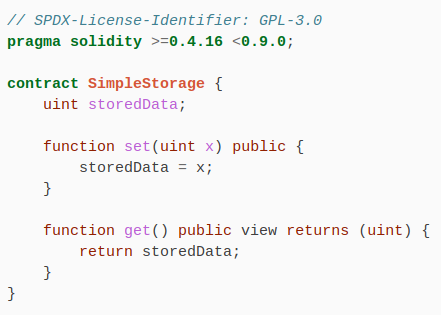
\includegraphics[width=0.5\textwidth]{./figs/smart-contract-example.png}
		\caption{Example of simple smart contract written in Solidity.}		
		\label{fig:smart-contract}
	\end{center}	
\end{figure}


\subsubsection{Data Types and
	Variables}\label{data-types-and-variables}

Solidity supports a rich set of data types, which can be broadly
classified into two categories:

\begin{itemize}
	\tightlist
	\item
	\textbf{Value Types}: These are data types that are passed by value,
	meaning that a copy of the value is created when it is assigned to a
	new variable or passed as an argument to a function. Value types
	include \texttt{bool}, \texttt{int}, \texttt{uint}, \texttt{address},
	and \texttt{bytes}.
	\item
	\textbf{Reference Types}: These are data types that are passed by
	reference, meaning that the new variable or function argument refers
	to the same location in memory as the original. Reference types
	include \texttt{arrays}, \texttt{structs}, and \texttt{mappings}.
\end{itemize}

Variables in Solidity can be stored in one of three data locations:

\begin{itemize}
	\tightlist
	\item
	\textbf{Storage}: This is the persistent storage of the contract,
	which is stored on the blockchain. State variables are stored in
	storage by default. It is the most expensive place in terms of gas since it is permanent.
	\item
	\textbf{Memory}: This is a temporary storage location that is cleared
	between function calls. It is used to store local variables and
	function arguments. In general, the memory is not permanent storage and thus operations with memory are cheap in terms of gas.
	\item
	\textbf{Calldata}: This is a read-only storage location that is used
	to store the input data for a function call. In fact, calldata location is also stored in memory and thus has the same cost implications in terms of gas.
\end{itemize}

\begin{center}\rule{0.5\linewidth}{0.5pt}\end{center}

\subsection{Functions and Control
	Structures}\label{section-2-functions-and-control-structures}

\subsubsection{Functions}\label{functions}

Functions are the fundamental units of execution in a Solidity smart
contract. They encapsulate the logic of the contract and can be called
either internally by other functions within the same contract or
externally by other contracts or users.

Solidity provides four visibility specifiers for functions, which
control how they can be accessed:

\begin{itemize}
	\tightlist
	\item
	\textbf{\texttt{public}}: Public functions can be called from
	anywhere, both internally and externally.
	\item
	\textbf{\texttt{private}}: Private functions can only be called from
	within the contract in which they are defined.
	\item
	\textbf{\texttt{internal}}: Internal functions can be called from
	within the contract in which they are defined and from any contracts
	that inherit from it.
	\item
	\textbf{\texttt{external}}: External functions can only be called from
	outside the contract.
\end{itemize}

In addition to visibility specifiers, functions can also have modifiers
that alter their behavior. The most common modifiers are:

\begin{itemize}
	\tightlist
	\item
	\textbf{\texttt{view}}: This modifier indicates that the function is
	read-only and does not modify the state of the contract.
	\item
	\textbf{\texttt{pure}}: This modifier indicates that the function does
	not read or modify the state of the contract.
	\item
	\textbf{\texttt{payable}}: This modifier indicates that the function
	can receive Ether.
\end{itemize}

Note that Solidity provides several globally available variables and functions that are specific either to the current transaction or the block in which the transaction is included. 
The most important such functions and variables are presented in \autoref{fig:special-vars} and \autoref{fig:special-vars2}.

\begin{figure}[t]
	%	\vspace{-0.3cm}
	\begin{center}
		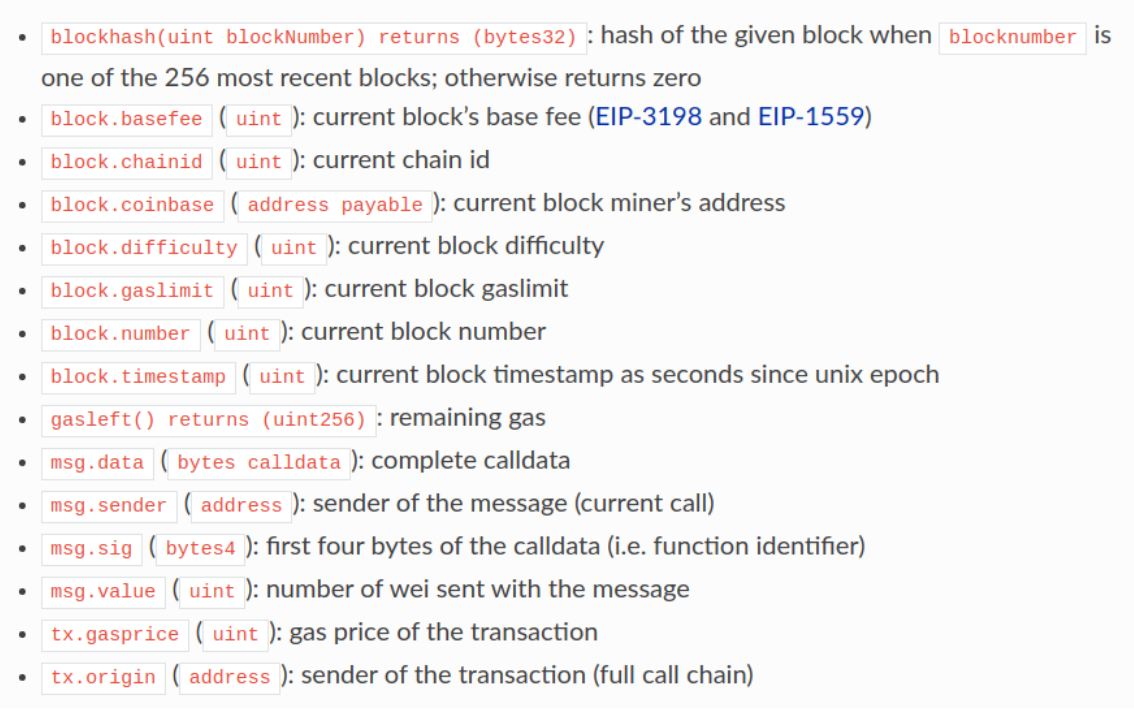
\includegraphics[width=0.9\textwidth]{./figs/vars-funcs.png}
		\caption{Globally available variables and functions.}		
		\label{fig:special-vars}
	\end{center}	
\end{figure}

\begin{figure}[t]
	%	\vspace{-0.3cm}
	\begin{center}
		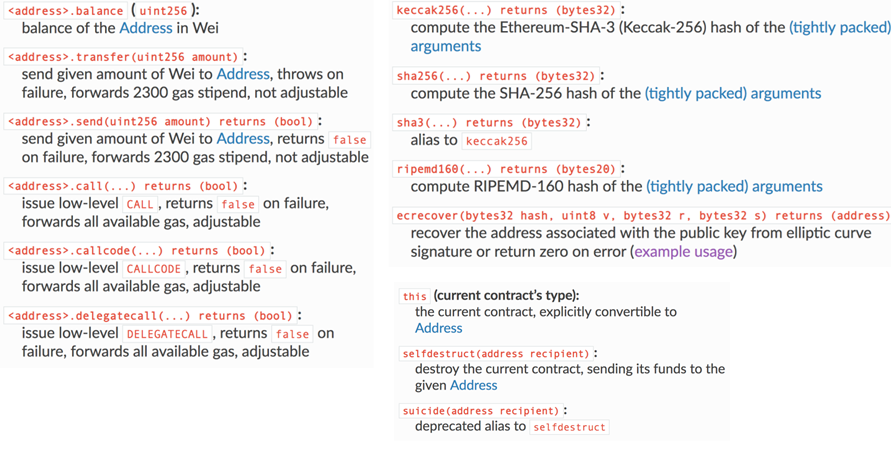
\includegraphics[width=0.99\textwidth]{./figs/functions2.png}
		\caption{Globally available variables and functions.}		
		\label{fig:special-vars2}
	\end{center}	
\end{figure}

\subsubsection{Control Structures}\label{control-structures}

Solidity supports a range of standard control structures that are common
to many programming languages, including:

\begin{itemize}
	\tightlist
	\item
	\textbf{Conditional statements}: \texttt{if}, \texttt{else}
	\item
	\textbf{Loops}: \texttt{while}, \texttt{for}, \texttt{do-while}
\end{itemize}

Solidity also provides three error-handling mechanisms that can be used
to revert the state of the contract if an error occurs:

\begin{itemize}
	\tightlist
	\item
	\textbf{\texttt{require}}: This function is used to validate inputs
	and conditions before executing a function. If the condition is not
	met, the transaction is reverted.
	\item
	\textbf{\texttt{assert}}: This function is used to check for internal
	errors and to validate invariants. If the condition is not met, the
	transaction is reverted.
	\item
	\textbf{\texttt{revert}}: This function is used to revert the
	transaction and provide an error message.
\end{itemize}

\subsubsection{\texorpdfstring{Special Functions: \texttt{receive}
		and
		\texttt{fallback}}{Special Functions: receive and fallback}}\label{special-functions-receive-and-fallback}

Solidity includes two special functions that are used to handle Ether
transfers and calls to non-existent functions:

\begin{itemize}
	\tightlist
	\item
	\textbf{\texttt{receive} function}: This function is executed when a
	contract receives a plain Ether transfer without any accompanying
	data. It must be declared as \texttt{external} and \texttt{payable}.
	\item
	\textbf{\texttt{fallback} function}: This function is executed when a
	contract receives a call to a function that does not exist in the
	contract. It can also be used to receive Ether if no \texttt{receive}
	function is defined.
\end{itemize}

These functions are essential for creating contracts that can interact
with the Ethereum network in a flexible and robust manner.


\subsubsection{Custom function modifiers}\label{sec:modifiers}
Solidity provides custom modifiers of functions that act in a similar fashion as macros in C/C++.
These custom modifiers are usually used to check authorization for calling the function or conditions to be met.
See two examples of custom function modifiers in \autoref{fig:modifiers}.

\begin{figure}[t]
	%	\vspace{-0.3cm}
	\begin{center}
		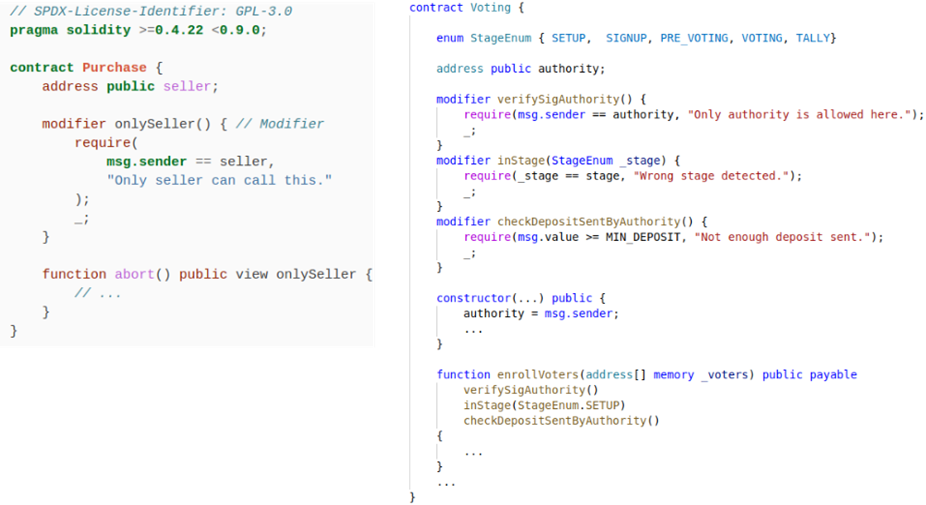
\includegraphics[width=0.9\textwidth]{./figs/modifiers-custom.png}
		\caption{Examples of custom function modifiers.}		
		\label{fig:modifiers}
	\end{center}	
\end{figure}

\subsubsection{Abstract contracts and interfaces}\label{sec:interfaces}
Similarly to  many other object-oriented programming languages, Solidity also supports abstract contracts and interfaces.
Contract is marked as abstract if at least one of its functions is not implemented. In contrast, interfaces must have not any function implemented.
See examples of abstract contract and interface in \autoref{fig:inteface}. 

\begin{figure}[bt]
	%	\vspace{-0.3cm}
	\begin{center}
		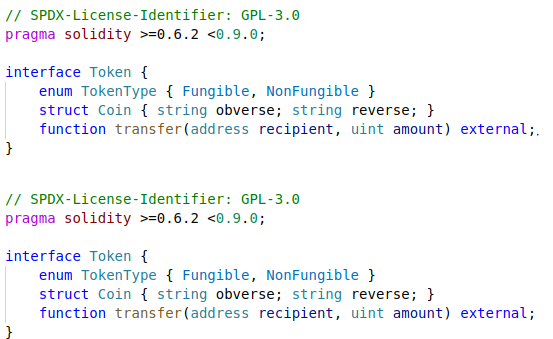
\includegraphics[width=0.7\textwidth]{./figs/abstract-contract.png}
		\caption{Examples of abstract contract and interface.}		
		\label{fig:inteface}
	\end{center}	
\end{figure}



\subsubsection{Libraries}\label{sec:libs}
Libraries are similar to contracts but they are deployed only once and their code is reused using the DELEGATECALL instruction.
If library functions are called, their code is executed in the context of the calling contract (especially modifying the storage of the calling contract).
Therefore, libraries are assumed to be stateless.
Libraries can be also seen as implicit base contracts of the contracts that use them.
An example of the library and its application to a specific data type is depicted in \autoref{fig:library}. 
Another example of library is depicted in \autoref{fig:library2}.


\begin{figure}[bt]
	%	\vspace{-0.3cm}
	\begin{center}
		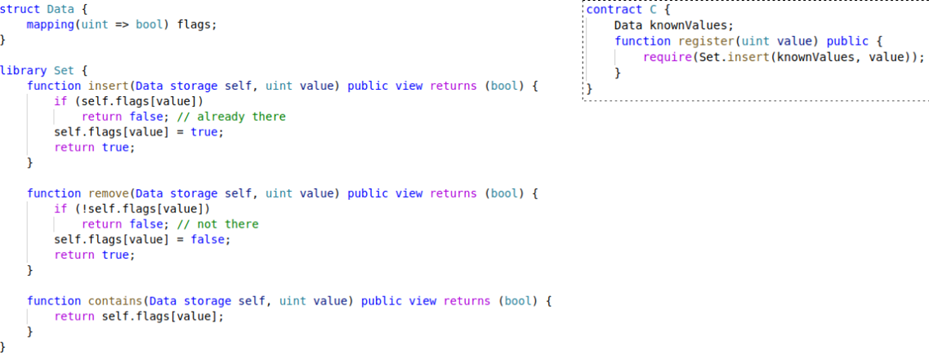
\includegraphics[width=0.99\textwidth]{./figs/library.png}
		\caption{The example of library contract and its application on a data type.}		
		\label{fig:library}
	\end{center}	
\end{figure}

\begin{figure}[bt]
	%	\vspace{-0.3cm}
	\begin{center}
		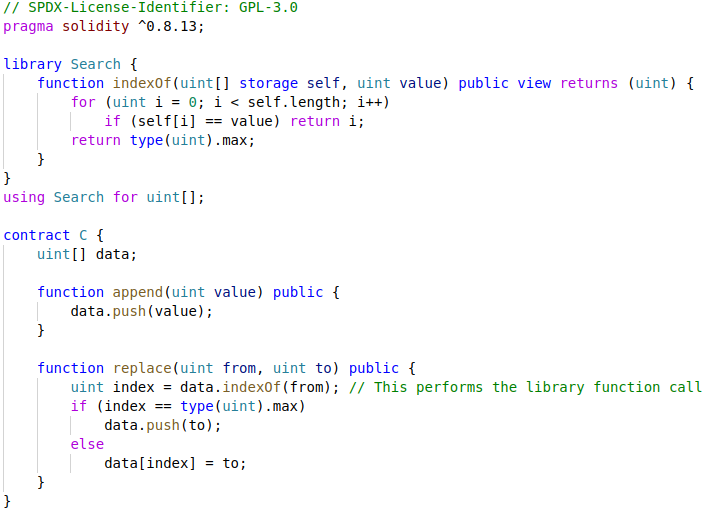
\includegraphics[width=0.8\textwidth]{./figs/library2.png}
		\caption{The example of library contract and its application using ``using'' and ``for''.}		
		\label{fig:library2}
	\end{center}	
\end{figure}



\begin{center}\rule{0.5\linewidth}{0.5pt}\end{center}

\subsection{Token Standards and Smart Contract
	Security}\label{section-3-token-standards-and-smart-contract-security}

\subsubsection{ERC20 and ERC721 Token
	Standards}\label{erc20-and-erc721-token-standards}

To promote interoperability and composability within the Ethereum
ecosystem, the community has developed a set of standards for different
types of tokens. The two most widely adopted standards are ERC20 and
ERC721.

\begin{itemize}
	\tightlist
	\item
	\textbf{ERC20}: This is the standard for fungible tokens, which are
	tokens that are identical and interchangeable. Examples of ERC20
	tokens include stablecoins like USDT and DAI, as well as governance
	tokens for various DeFi protocols. The ERC20 standard defines a common
	interface that includes functions for transferring tokens, checking
	account balances, and approving other accounts to spend tokens on
	behalf of the owner.
	The interface of ERC20 contract is depicted in \autoref{fig:erc20}.
\end{itemize}

\begin{figure}[t]
	%	\vspace{-0.3cm}
	\begin{center}
		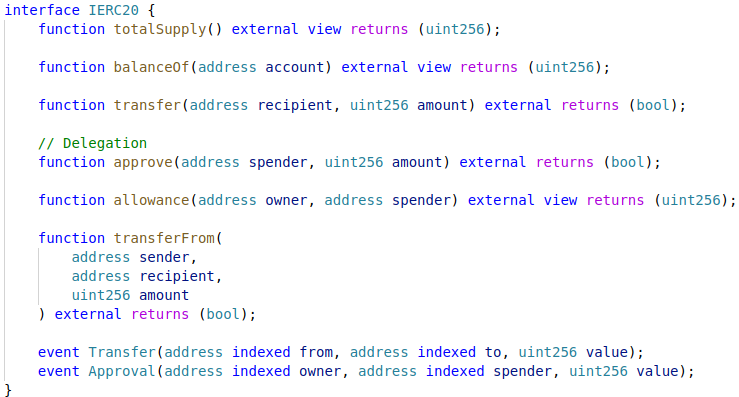
\includegraphics[width=0.9\textwidth]{./figs/ERC20.png}
		\caption{ERC20 interface.}		
		\label{fig:erc20}
	\end{center}	
\end{figure}
\begin{figure}
	%	\vspace{-0.3cm}
	\begin{center}
		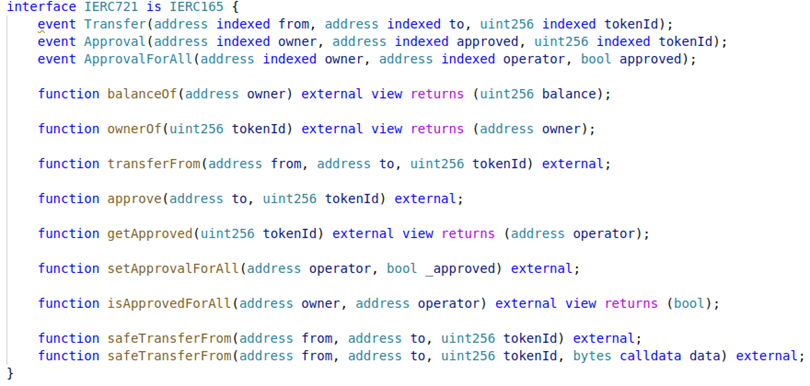
\includegraphics[width=0.9\textwidth]{./figs/ERC721.png}
		\caption{ERC721 interface.}		
		\label{fig:erc721}
	\end{center}	
\end{figure}


\begin{itemize}
	\tightlist
	\item
	\textbf{ERC721}: This is the standard for non-fungible tokens (NFTs),
	which are unique and non-interchangeable. Each ERC721 token has a
	unique ID and can be used to represent a wide range of assets, from
	digital art and collectibles to real estate and intellectual property.
	The ERC721 standard defines a common interface for tracking the
	ownership of each individual token.
	The interface of ERC721 contract is depicted in \autoref{fig:erc721}.
\end{itemize}




These token standards have been instrumental in the growth of the
Ethereum ecosystem, as they allow for seamless integration between
different applications, such as wallets, exchanges, and DeFi protocols.




\clearpage
\subsubsection{Smart Contract
	Security}\label{smart-contract-security}

The immutable nature of blockchains means that bugs and vulnerabilities
in smart contracts can have severe and irreversible consequences, often
leading to significant financial losses. Therefore, smart contract
security is of paramount importance. Some of the most common security
vulnerabilities include:

\begin{itemize}
	\tightlist
	\item
	\textbf{Reentrancy Attacks}: This is a type of attack where a
	malicious contract can repeatedly call a function on a victim contract
	before the first call has completed. This can be used to drain funds
	from the victim contract if it does not follow the
	checks-effects-interactions pattern. The infamous DAO attack was a
	result of a reentrancy vulnerability (see \autoref{fig:dao-bug}).
\end{itemize}


\begin{figure}[t]
	%	\vspace{-0.3cm}
	\begin{center}
		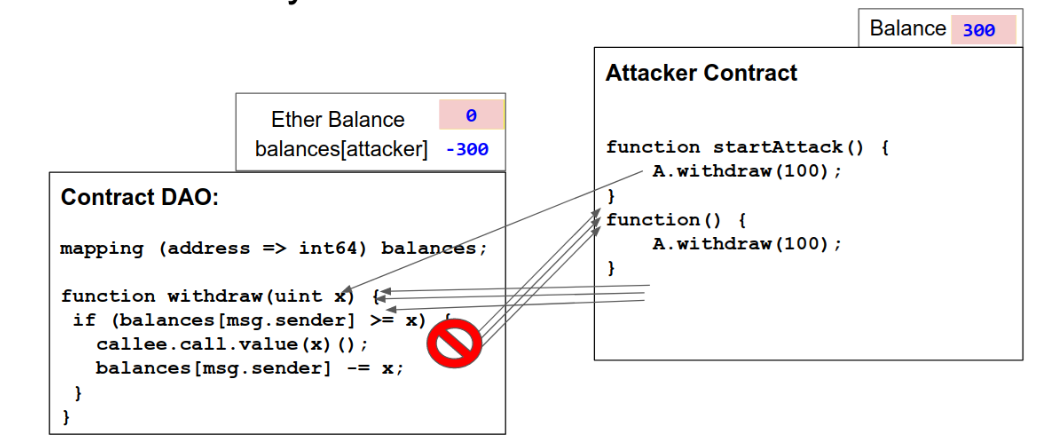
\includegraphics[width=0.9\textwidth]{./figs/DAO.png}
		\caption{Reentrancy vulnerability in DAO bug.}		
		\label{fig:dao-bug}
	\end{center}	
\end{figure}

\begin{itemize}
	\tightlist
	\item
	\textbf{Integer Overflows and Underflows}: These vulnerabilities occur
	when an arithmetic operation results in a value that is outside the
	range of the data type. This can lead to unexpected behavior and can
	be exploited by attackers to manipulate the state of the contract.
	It can, for example, cause out of gas exception due to comparing mismatching data types:  \verb| for (var i = 0; i < 2000; i++) { ... } |. Note that i is of type uint8 and thus will never reach the value 2000.
	
%	\begin{figure}[t]
%		%	\vspace{-0.3cm}
%		\begin{center}
%			\includegraphics[width=0.8\textwidth]{./figs/underflow.png }
%			\caption{Out of gas exception due to integer underflow.}		
%			\label{fig:underflow}
%		\end{center}	
%	\end{figure}
	
	\item
	\textbf{Denial-of-Service (DoS) Attacks}: An attacker can exploit
	certain vulnerabilities to render a contract unusable, for example, by
	causing it to run out of gas or by making it impossible for other
	users to interact with it.
\end{itemize}

Another notable example of smart contract vulnerabilities is the Parity
Wallet bug, which led to the freezing of millions of dollars worth of
Ether. This bug was caused by a flaw in the way the wallet's library
contract was initialized, allowing an attacker to take ownership of the
library and self-destruct it.

\subsubsection{Upgradeable Smart
	Contracts}\label{upgradeable-smart-contracts}

While smart contracts are immutable by default, there are scenarios
where it is desirable to be able to modify them, for example, to fix a
bug or to add new functionality. The Proxy and Implementation pattern is
a common approach to creating upgradeable smart contracts. This pattern
involves a proxy contract that stores the state of the contract and
delegates all calls to an implementation contract (see \autoref{fig:upgradable}). The implementation
contract can be replaced with a new version without affecting the state
of the proxy contract.

\begin{figure}[t]
	%	\vspace{-0.3cm}
	\begin{center}
		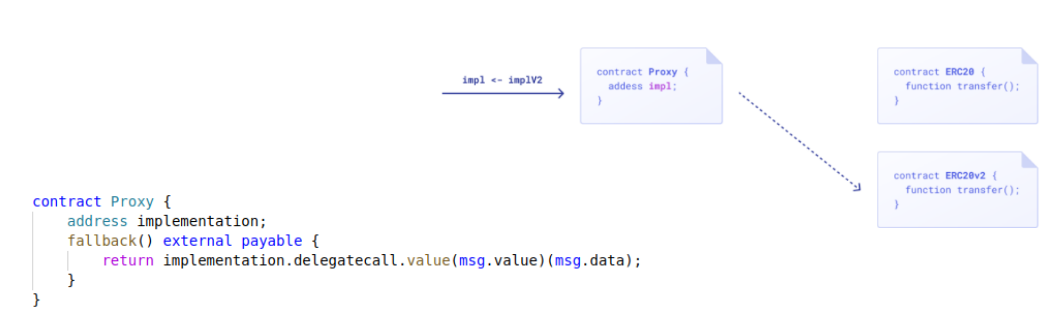
\includegraphics[width=0.99\textwidth]{./figs/upgradable.png}
		\caption{Proxy and implementation pattern.}		
		\label{fig:upgradable}
	\end{center}	
\end{figure}


\subsubsection{Tools for Smart Contract Development and
	Analysis}\label{tools-for-smart-contract-development-and-analysis}

A rich ecosystem of tools has emerged to support the development and
analysis of secure and robust smart contracts. These tools can be
broadly categorized as follows:

\begin{itemize}
	\tightlist
	\item
	\textbf{Development Frameworks}: These provide a comprehensive
	environment for compiling, testing, and deploying smart contracts.
	Popular frameworks include Truffle and Hardhat.
	\item
	\textbf{Browser-Based IDEs}: These provide a convenient and
	user-friendly environment for writing and testing smart contracts
	directly in the browser. Remix is the most widely used browser-based
	IDE.
	\item
	\textbf{Static Analysis Tools}: These tools analyze the source code of
	a smart contract to identify potential vulnerabilities and deviations
	from best practices. Examples include Slither and Solhint.
	\item
	\textbf{Dynamic Analysis Tools}: These tools analyze the behavior of a
	smart contract as it is being executed to identify vulnerabilities
	that may not be apparent from a static analysis. Examples include
	Echidna and Manticore.
\end{itemize}

\begin{center}\rule{0.5\linewidth}{0.5pt}\end{center}

\subsection{Summary / Key Takeaways}\label{summary-key-takeaways}

This section has provided a practical, hands-on introduction to the
world of smart contract programming with Solidity. We have covered the
essential elements of the language, from its basic syntax and data types
to its more advanced features, such as function modifiers and visibility
specifiers.

We have explored the structure of a Solidity contract and the different
data locations that can be used to store variables. We have also
examined the role of special functions like \texttt{receive} and
\texttt{fallback} in handling Ether transfers and interacting with other
contracts.

A key focus of this section has been on the practical application of
Solidity. We have discussed the ERC20 and ERC721 token standards, which
are the foundation of the vibrant DeFi and NFT ecosystems on Ethereum.

Finally, we have addressed the critical importance of smart contract
security. We have identified common vulnerabilities, such as reentrancy
attacks and integer overflows, and we have highlighted the tools and
best practices that developers can use to write secure and robust code.

By the end of this section, you should have a solid foundation in smart
contract programming and be well-equipped to start building your own
decentralized applications on the Ethereum blockchain.

\begin{center}\rule{0.5\linewidth}{0.5pt}\end{center}

\subsection{Keywords}\label{keywords}

\begin{itemize}
	\tightlist
	\item
	\textbf{Solidity}: A high-level, object-oriented programming language
	for writing smart contracts on the Ethereum blockchain.
	\item
	\textbf{Smart Contract}: A self-executing contract with the terms of
	the agreement between buyer and seller being directly written into
	lines of code.
	\item
	\textbf{ERC20}: A technical standard used for smart contracts on the
	Ethereum blockchain for implementing tokens.
	\item
	\textbf{ERC721}: A standard for non-fungible tokens (NFTs) on the
	Ethereum blockchain.
	\item
	\textbf{Reentrancy}: A common smart contract vulnerability where a
	malicious contract can repeatedly call a function on a victim contract
	before the first call has completed.
	\item
	\textbf{Visibility Specifiers}: Keywords in Solidity that control the
	accessibility of functions and state variables.
	\item
	\textbf{Function Modifiers}: Reusable pieces of code that can be used
	to change the behavior of functions in a declarative way.
	\item
	\textbf{Truffle}: A popular development framework for Ethereum that
	provides a suite of tools for compiling, testing, and deploying smart
	contracts.
	\item
	\textbf{Hardhat}: A flexible and extensible Ethereum development
	environment that is widely used for smart contract development.
	\item
	\textbf{Remix}: A browser-based IDE for Solidity that provides a
	convenient environment for writing, testing, and deploying smart
	contracts.
\end{itemize}

\begin{center}\rule{0.5\linewidth}{0.5pt}\end{center}

\subsection{Further Reading}\label{further-reading}

\begin{itemize}
	\tightlist
	\item
	\textbf{Solidity Documentation}: \\
	\url{https://docs.soliditylang.org/}
	\item
	\textbf{OpenZeppelin Contracts}: \\
	\url{https://github.com/OpenZeppelin/openzeppelin-contracts}
	\item
	\textbf{ConsenSys Smart Contract Best Practices}: \\
	\url{https://consensys.github.io/smart-contract-best-practices/}
\end{itemize}
